\documentclass{article}
\usepackage{amsmath,amsfonts,amsthm,amssymb,wasysym}
\usepackage{setspace}
\usepackage{enumitem}
\usepackage{Tabbing}
\usepackage{fancyhdr}
\usepackage{lastpage}
\usepackage{chngpage}
\usepackage{url}
\usepackage{subfigure}
\usepackage{array}
\usepackage{multicol}
\usepackage[color=blue!40]{todonotes}
\usepackage[protrusion=true,expansion,kerning]{microtype}
\usepackage{natbib}

% to adjust margins:
\topmargin=-0.25in
\evensidemargin=0in
\oddsidemargin=0in
\textwidth=6.25in
\textheight=8.5in
\headsep=0.25in

% homework specific information
\newcommand{\hmwkTitle}{Machine Learning Paper}
\newcommand{\hmwkDueDate}{December 6, 2013}
\newcommand{\hmwkClass}{}
\newcommand{\hmwkClassInstructor}{}
\newcommand{\hmwkAuthorName}{Sullivan, Cellier, Hobbs}

% math aliases
\newcommand{\reals}{\mathbb{R}}
\newcommand{\twopartdef}[4]
{
	\left\{
		\begin{array}{ll}
			#1 & \mbox{if } #2 \\
			#3 & \mbox{if } #4
		\end{array}
	\right.
}

% header and footer
\pagestyle{fancy}
\lhead{\hmwkAuthorName}
\chead{\hmwkTitle}
\rhead{\hmwkDueDate}   
\lfoot{}
\cfoot{}
\rfoot{\emph{Page\ \thepage\ of\ \pageref{LastPage}}}                          
\renewcommand\headrulewidth{0.4pt}
\renewcommand\footrulewidth{0.4pt}

\makeatletter
\newenvironment{tablehere}
  {\def\@captype{table}}
  {}

\newenvironment{figurehere}
  {\def\@captype{figure}}
  {}
\makeatother

%\renewcommand{\bibsection}{\subsubsection*{\refname}}

% Make title 
\title{
\LARGE\bf Patent Classification using Supervised Methods \\
\date{}
\author{ John Sullivan \and Caitlin Cellier \and J. Nicholas Hobbs}
}

\begin{document}

\maketitle

%%%%%%%%%%%%%%%%%%%%%%%%%%%%%%%%%%%%%%%%%%%%%%%%%%%%%%%%%%%%%%%%%
\begin{abstract}
Recent studies have suggested the brain is composed of clusters that are in communication with each other. Using this as a basis, we propose a feed-forward neural network that is formed with clusters instead of individual neurons at each layer. Preliminary results suggest that this type of network has detrimental effects on the rate of network accuracy and convergence. Further work should be done to create a better model of these recent studies of the brain.
\end{abstract}
%%%%%%%%%%%%%%%%%%%%%%%%%%%%%%%%%%%%%%%%%%%%%%%%%%%%%%%%%%%%%%%%%


\thispagestyle{fancy}

\maketitle

%%%%%%%%%%%%%%%%%%%%%%%%%%%%%%%%%%%%%%%%%%%%%%%%%%%%%%%%%%%%%%%%%
\section{Introduction}
The United States Patent Office granted 276,788 patents in 2012\cite{USPTO:2013:stats}. This is more than double the number granted 20 years ago, and rate of filings is still increasing. In the circumstance it makes sense to consider scalable, automated approaches to parts of the patent review process. To this end we examined both attempting to classify patents into existing categorizations using supervised machine learning techniques, and creating alternative categorizations using unsupervised machine learning techniques. We also attempted to measure the coherency of the existing classifications. Reliable automation of patent categorization is an important first step to larger scale automation of the patent review process.



Specifically, we considered the use of machine learning classifiers to automatically categorize patents into each of the 8 patent categories specified in the International Patent Classification\cite{ipc:2013:guide}. The USPTO is moving from its previous classification system (which contained thousands of classes and was deemed unusable for this project) to the Cooperative Patent Classification, which is a superset of the IPC. US patent grants since <FIND A YEAR> have been labelled with an IPC Classification in preparation for this turn over.

% multiple categories can be assigned
% CPC has cross-category
% Break out category talk to separate section/move to dataset
% talk more about size of task and need for speed

% Difference between CPC and IPC
% Relative size of categories?

\begin{table}[H]
	\centering
	\begin{tabular}{ | l | l |}
		\hline
		\textbf{Class} & \textbf{Title} \\
				\hline
		A & Human Necessities \\
				\hline
		B & Performing Operations; Transporting \\
				\hline
		C & Chemistry; Metallurgy \\
				\hline
		D & Textiles; Paper \\
				\hline
		E & Fixed Constructions \\
				\hline
		F & Mechanical Engineering; Lighting; Heating; Weapons; Blasting Engines or Pumps \\
		\hline
		G & Physics \\
				\hline
		H & Electricity \\
				\hline
	\end{tabular}
	\caption{IPC Classifications and their titles}
\end{table}



%Many of these patents are awarded to so-called nonpracticing entities (NPEs), organizations that do not design, build (or even prototype) the techniques and technologies under patent, but rather create or invest in patent portfolios to litigate against organizations or individuals that build related products. At the same time, patent litigation has been increasing, particularly litigation initiated by NPEs\cite[p. 7]{PWC:2013:lit}. In such an environment, it is more important than ever to be able to quickly and reliably assess the quality of patents, both in terms of their content, and whether they represent truly original work. 

% More Here!!

%The structure of the brain influences availability and access to the memories stored therein. Communication between neurons allows animals to think, move, and store or recall memories. It seems plausible that the structure of an artificial neural network would similarly affect the ability of that neural network to store and process information. Building off this idea, we suggest a new model of neural network influenced by Perin, Berger, and Markram (2011) who proposed that the brain is composed of a hierarchy of connected components with specific associated computational functions. 

%We implemented this model within the framework of deep learning inspired by Hinton (2007).  More specifically, we describe a model of deep learning based on the use of acyclic clusters which mimic multiple layers of neurons. Additionally, these clusters themselves are layered. We found that this model did not significantly increase the ability of our network to generate or classify handwritten digits, nor did it increase the computational efficiency of those tasks.
%\label{sec:Introduction}
%%%%%%%%%%%%%%%%%%%%%%%%%%%%%%%%%%%%%%%%%%%%%%%%%%%%%%%%%%%%%%%%%

%Some text, cite this~\cite{ASBMI,Acharya07}, and also Figure~\ref{fig:something}.
\section{Data Set and Feature Selection}
%\cite*{mimno-mccallum-11}

\subsection{Dataset Construction}
\indent
The United States Patent Office makes bulk patent grant information available through several private companies\cite{USPTO:2013:patent-catalog} in XML format\cite{USPTO:2013:dtd}. For our experiments we drew samples from patent grants made between May 1st 2012 and July 31st 2012. Over these three months the USPTO granted a total of 76,317 patents, or roughly 6,000 per week. We constructed three datasets from this, \emph{even-3500}, \emph{jagged-20000}, and \emph{jagged-40000}. \emph{even-3500} consisted of 350 training and 150 test instances from 7 of the 8 IPC patent classes (one class, D, which corresponds to textiles and paper could not be used since a only 47 patents were granted to that section in our dataset). \emph{jagged-20000} and \emph{jagged-40000} were simply a random sample of 20,000 and 40,000 patents respectively granted within the given timeframe, using all 8 of the IPC patent classes.

\subsection{Feature Selection}
\indent
Patents are semi-structured. That is, rather than simply being free text, there are certain fields that all patent grants are guaranteed to have (as well as other, optional fields). This needs to be taken into consideration when designing features for patent classification. 

Although a domain expert could potentially design features that were powerful, we ended up considering three relatively general feature sets, \emph{description-unigrams}, \emph{abstract-bigrams}, and \emph{tf-idf}. \emph{description-unigrams} consists of unigrams from the main ``description'' field of the patent document, tokenized and with stopwords removed. \emph{abstract-bigrams} consists of unigrams and bigrams from the ``abstract'', ``claims'', and ``title'' fields of the patent. \emph{tf-idf} consists of the tokens (and token-pairs) from \emph{abstract-bigrams} weighted them with a statistic called term frequency inverse document frequency (TFIDF)\cite{manning:2008:IR}. Intuitively, the TFIDF weight of a token (or token bigram) in a document increases as the number of times it occurs in that document increases and decreases as the number of times it appears in every other document increases. This weighting gives us a sense of how characteristic the token (or token bigram) is of each document. Once we calculated TFIDF scores for each document, we truncated the word bags to contain only the 32, 100, and 200 highest weighted features for each patent. We used tools in FACTORIE\cite{mccallum09:factorie:} to tokenize the patents and remove stopwords. We also added domain-specific stopwords based on observations of patent documents. 

Both of these bag of n-grams models can be easily translated into vectors. This allows us to use a variety of standard machine learning multiclass classification techniques. For some set of documents $\mathbf{D}$, let $| \mathbf{V} |$ denote the number of unique n-grams that appear in that set of documents (for a given tokenizer and stopword lexicon). Then we can represent each document $ d \in \mathbf{D}$ by a binary vector $f \in \{0,1\}^{| \mathbf{V} |}$, where $f^d_i = 1$ when $d$ contains the $i$\textsuperscript{th} n-gram in the vocabulary and 0 otherwise. Nominally, these feature vectors are very large ($| \mathbf{V} | > 900000$ for \emph{abstract-bigrams} on \emph{jagged-40000}). Thus we need to represent these vectors sparsely in practice in order to work tractably with them.


%Our data is from the United States Patent and Trademark Office Bulk Downloads located on Google.  The original data file is prepared as an XML file, which we then parse to find a list of words contained within the patent.  Based on the total list of words of all patents in a sample, a feature vector is created such that the feature vector includes a feature for every seen word within the dataset.  A 1 is included for a feature within a feature vector for a patent if the patent contains the word, and a 0 is included for a specific feature if the patent did not include the word.  This bag of words technique was used for all experiments.
\section{Classification Techniques}
%%Just have dataset here instead of a whole separate section? If it's in it's own section then we can give a fuller background on the classes and maybe an explanation of the coherence scores
%\subsection{Data Set}

\subsection{Maximum Entropy} % (fold)
\label{sub:maximum_entropy}
A maximum entropy classifier calculates a probability distribution over label classes conditioned on the observed feature vector. Usually the predicted class of a feature vector is taken to be the class with the highest probability under a learned parameterization of the distribution. The learning step simply involves estimating the natural parameters of an exponential distribution. Customarily the observed feature vector is binary. Taking $f^d$ to represent the feature vector for a single document, as above, $y$ to be the class we want to predict, and $\theta$ to be the weight vector we want to learn, this gives
\begin{align*}
	P(y|f, \theta) = \frac{e^{\theta \cdot f}}{\sum_{f'} e^{\theta \cdot f'}}
\end{align*}

We can estimate the parameters of this distribution easily using standard convex optimization techniques. Since this distribution is a natural formulation of the exponential family, it is the distribution that highest entropy subject to the constraints imposed by the observed feature vectors, hence its name. For this paper we used the Maximum Entropy model implemented in FACTORIE.

% subsection maximum_entropy (end)

\subsection{Multiclass SVM} % (fold)
\label{sub:multiclass_svm}


% subsection multiclass_svm (end)


%\subsection{Supervised Methods}
%For the first experiment, the dataset was created such that each of the 7 classification categories were evenly represented with 200? samples each.  (Define Training/Testing and re-run experiment)

Description of SVM -------



%% Tempted to make this it's own section as well
\subsection{Dimensionality Reduction}

Description of PCA and Laplacian


For the second experiment, the dataset from experiment one had two different dimensionality reduction techniques used to reduce the dataset.  The two included PCA and a Laplacian Eigenmap.  (Define Training/Testing and re-run experiment)
\subsection{Boosting Methods}
For the third experiment, we attempted to determine if more data would noticeably improve the results of the algorithm.  Specifically, the dataset was expanded to approximately 2000 samples each. (Define Training/Testing and re-run experiment)
\section{Results}
\subsection{Baseline}
For our first test we need to establish a baseline to compare all other results against.  We use the \emph{even-3500} dataset which included  \emph{description-unigrams} for this baseline.  A support vector machine and maximum entropy algorithm were trained on this dataset.  The support vector machine attained 49.33\% for its testing accuracy. The testing accuracy for maximum entropy was 46.12\%.  Because there are 7 categories, random chance would put the accuracy at 14.28\%.  This means that, as a baseline, the algorithms are already performming above random chance.

\subsection{Dimensionality Reduction}
Due to the large number of features, we first attempted dimensionality reduction on the dataset as a means to increase the accuracy of the algorithm.  We attempt two dimensionlaity reductions, principle component analysis and laplacian eigenmap. Both processes were applied to the \emph{even-3500} dataset of \emph{descrption-unigrams}.  We found that the results tended to be ambiguous, in that the testing accuracy of maximum entropy tended to increase by approximately 7\% while the support vector machine had its testing accuracy decreased by 7\%.  However, except for these adjustments, the results did not change significantly.
\\

\begin{figure}[!h]
\begin{center}
\caption{Maximum Entropy with Dimensionality Reduction Testing Accuracy}
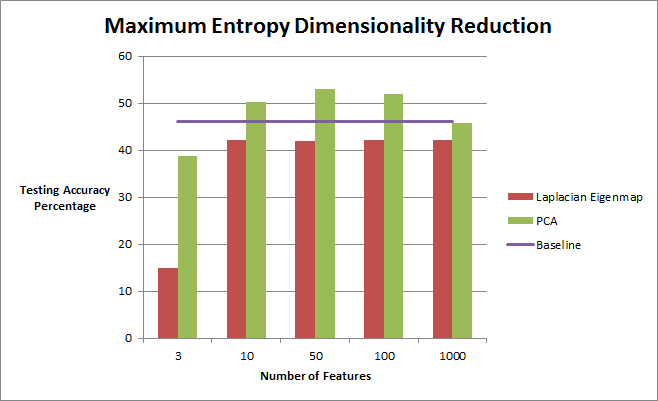
\includegraphics[width=0.7\textwidth]{Maximum_Entropy_Dimensionality_Reduction.png}
\end{center}
\end{figure}

\begin{figure}[!h]
\begin{center}
\caption{SVM with Dimensionality Reduction Testing Accuracy}
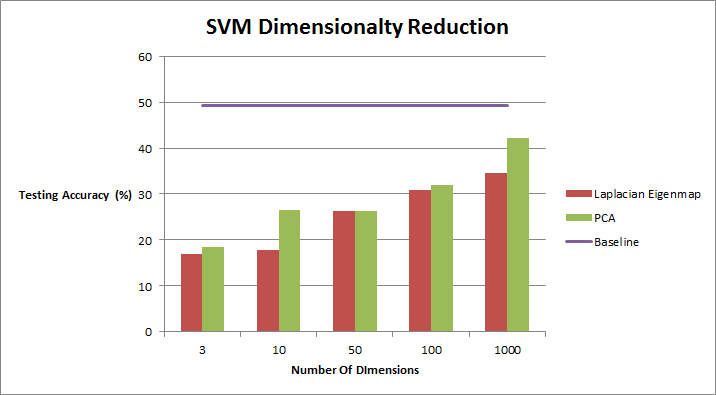
\includegraphics[width=0.7\textwidth]{SVM_Dimensionality_Reduction.png}
\end{center}
\end{figure}

Overall, it is interesting to note that there tended to be early convergence in the number of features.  Specifically, maximum entropy converged by around the 10 dimensionality mark, and the difference between 100 and 1000 for the support vector machine was significant for PCA, however, it was not significant for the Laplacian eigenmapA.  This seems to suggest that in natural language tasks, dimensionality reduction quickly converges to find the important features that should be used in data processing.  Though this is an interesting result, to have an accurate comaprison against our baseline, further results do not include dimensionality reduction and focus instead on dataset size and feature selection.  Intuitively, because PCA tended to have a higher testing accuracy, it is suggestive that focusing on the variance of the problem was more important than attempting to keep the local proximity of the inputs constant.

\subsection{Dataset Size}
For the third set of experiments we wanted to determine to what extent more data would begin to alter the accuracy the algorithms.  We use the the \emph{jagged-20000} and \emph{jagged-40000} datasets which each included \emph{description-unigrams}.

\begin{figure}[!h]
\begin{center}
\caption{Testing Accuracy with \emph{description-unigrams} features}
\begin{tabular}{| r | c | c |}
\hline
\textbf{Dataset} & \textbf{SVM} & \textbf{Maximum Entropy} \\ \hline
\emph{even-3500} & 49.33\% & 46.12\% \\ \hline
\emph{jagged-20000} & 66.8667\% & 69.21\% \\ \hline
\emph{jagged-40000} & 69.53\% & 69.75\% \\ \hline
\end{tabular}
\end{center}
\end{figure}

The size of the dataset noticeably improved the results from 3500 to 20000.  However, after this point it appears that the algorithm converged.  This is seen from the change from 20000 to 40000 samples.  The increase was nearly insignificant for the maximum entropy algorithm.  To summarize, data is able to improve the testing accuracy up to a point, then gains are very small in comparison to early gains.  To further improve the results, either a different classification algorithm would need to be used, or a different set of features would need to be included.  To this end, the following set of experiments will attempt new ways of calculating the feature-vectors for each patent within the \emph{jagged-40000} dataset used in this experiment.

\subsection{Abstract Bigrams}
For the fourth experiment, the \emph{jagged-40000} dataset was used with \emph{abstract-bigrams} used as the features.  The results indicate that the support vector machine had an accuracy of 72.12\% and the maximum entropy algorithm had an accuracy of 72.57\%.  Overall, this is a slight improvement from experiment 3 of 3\% for the support vector machine and an increase of 3\% for the maximum entropy classifier.

\begin{figure}[!h]
\begin{center}
\caption{SVM with Dimensionality Reduction Testing Accuracy}
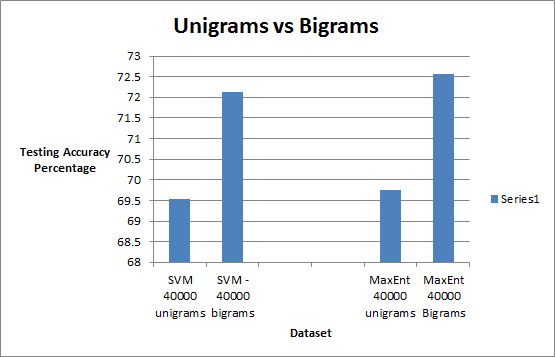
\includegraphics[width=0.7\textwidth]{Unigrams_vs_Bigrams.png}
\end{center}
\end{figure}

The small gains from this experiment are strictly due to the use of \emph{abstract-bigram} features.  This is known from the fact that only item which changed between the \emph{jagged-40000} dataset in the previous set of experiments was the move from \emph{description-unigrams} to \emph{abstract-bigrams}.  These results seem to suggest that it is still possible that further gains can be made by creating better features. Therefore, it is still of interest to attempt to create more intelligent features while using the largest possible dataset that we have.  The next experiment will attempt this experiment. 

\subsection{tf-idf}
We then used \emph{tf-idf} on the \emph{jagged-40000} dataset.  The results showed a noticeable improvement from the original dataset, however only a slight improvement from the abstract-bigrams.  Specifically, the score for the support vector machine was nearly identical to the abstract-bigrams, and maximum entropy increased by ~5\% from the baseline results.

\begin{figure}[!h]
\begin{center}
\caption{tf-idf for jagged-40000 features}
\begin{tabular}{| r | c | c |}
\hline
\textbf{Features} & \textbf{SVM} & \textbf{Maximum Entropy} \\ \hline
32 & 54.37\% & 66.79\% \\ \hline
100 & 63.62\% & 71.84\% \\ \hline
250 & 72.1\% & 74.15\% \\ \hline
\end{tabular}
\end{center}
\end{figure}

\emph{tf-idf} is a more abstract set of features tha are built off of \emph{the abstract-bigrams}.  These more abstract features are more intelligent created, and the results of these features were able to further increase the accuracy of the testing algorithm for maximum entropy.  It is interesting to note, however, that the support vector machine did not gain a boost in accuracy as maximum entropy did.  Furthermore, the results gained from these features for maximum entropy were only ~2\%.  These small gains are suggestive that more intelligent features are, in fact, able to improve the results, however with more intelligent features the gains are beginning to decline.  It would still be interesting to attempt different features to determine if this trend holds, however, this set of abstract features did perform the best out of all other sets of features we had tested.

\subsection{Summary}

These results have a few interesting findings.  First, dimensionality reduction is able to converge quite early in terms of the dimensionality of the vectors after the process.  This is noted by maximum entropy converging early in the process, and the laplacian eigenmap for the support vector machine showing early convergence.  
\\A second finding is regarding the sample size used for the patents.  It is interesting to note that the jump from 3500 samples to 20000 samples noticealby imrpoved the algorithm.  However, after that point, the algorithm did not gain in its testing accuracy.  This is suggestive that even when samples are doubled, results will have a tendency to converge.  This is suprising given the fact we had initially expected the results to continue to improve has more data was included.
\\Finally, the last finding of the results are regarding the abstractness of features.  \emph{description-unigrams} did the worst out of all possible sets of features in the construction of feature-vectors.  However, as the features tended to become more abstract in terms of one set of features being built off of an early set, the testing accuracy of the algorithms further improved.  This is noted by the move to \emph{abstract-bigrams} from \emph{description-unigrams} improving the testing accuracy, and furthermore the move from tf-idf being built with \emph{abstract-bigrams} have a higher testing accuracy than only the \emph{abstract-bigrams}. Overall, we found these finding to be interesting, and a few of them even surprising.
%%%%%%%%%%%%%%%%%%%%%%%%%%%%%%%%%%%%%%%%%%%%%%%%%%%%%%%%%%%%%%%%%
\section{Contributions}
\label{sec:Contributions}
%%%%%%%%%%%%%%%%%%%%%%%%%%%%%%%%%%%%%%%%%%%%%%%%%%%%%%%%%%%%%%%%%

We did good things
%\section{Previous Work}


%\begin{multicols}{1}



\bibliography{Sullivan_Cellier_Hobbs}
\bibliographystyle{unsrt}

%\end{multicols}

\end{document}